\documentclass[10pt]{article}

\usepackage[a4paper,top=2cm,bottom=2cm,left=2.2cm,right=2.2cm]{geometry}
\usepackage{amsmath,amssymb,amsthm}
\usepackage{booktabs}
\usepackage{graphicx}
\usepackage{microtype}
\usepackage[hidelinks]{hyperref}
\usepackage[numbers,sort&compress]{natbib}
\usepackage{xcolor}

\newtheorem{definition}{Definition}
\newtheorem{problem}{Problem}

\title{\textbf{Multi-Resolution Semantic Abstraction\\over an Evolving Knowledge Hypergraph}}
\author{Ali Rastegar Mojarad \\ \small Constructor Knowledge Labs}
\date{\today}

\begin{document}
\maketitle

% ─────────────────────────────────────────────────────────────
\begin{abstract}
We build a four-level topic hierarchy over a Temporal Knowledge Hypergraph (TKH)
of materials-science literature: 5,798 nodes and 1,429 hyper-edges from 52 papers,
organised into 12$\to$60$\to$300$\to$leaf super-nodes at four time snapshots
($\leq$2020, 2022, 2024, 2026).
The method combines sentence-embedding similarity ($\alpha=0.6$) with
arity-weighted co-occurrence ($0.4$) and uses Ward-linkage agglomerative clustering.
Hyper-edges are coarsened natively at every level — no pairwise projection.
Temporal stability is maintained by reusing cached embeddings for existing nodes
and tracking 327 lifecycle events (birth/growth/death/\ldots) via Jaccard matching.
Coherence, measured with an \emph{independent} embedding model (mpnet) to avoid
circularity, sits 60–243 standard deviations above a random null model.
Perturbation ARI (10\% edge removal, 5 seeds) is 0.67–0.88 with 95\% CIs.
Label over-claim rate is 1.4–8.3\% (GPT-4o-mini blind judge).
Drill-down retrieval on the 17-question benchmark slightly beats flat search
(HR@10: 0.132 vs.\ 0.123); the main value is navigability, not raw recall.
\end{abstract}

\begin{center}
  \small Code and data: \url{https://github.com/4lirastegar/multi-resolution-tkh}
\end{center}


% ─────────────────────────────────────────────────────────────
\section{Problem Statement}\label{sec:formal}

The TKH stores scientific literature as a \emph{hypergraph}: nodes are entities
(methods, datasets, authors, claims, \ldots) and edges connect three or more nodes
at once — a single edge can encode ``method $M$ was evaluated on dataset $D$ using
metric $Q$ in paper $P$''.
With $\sim$5,800 nodes, flat enumeration is useless.
We need a \emph{multi-resolution view}: roughly a dozen macro-topics at the top,
drilling down to individual nodes at the bottom — and stable as the corpus grows.

\begin{definition}[TKH snapshot]
$H(t) = (V(t), E(t))$ where $E(t) = \{e : \mathrm{year}(e) \le t\}$ and
$V(t) = \bigcup_{e \in E(t)} M(e)$.
A node enters the snapshot only once a paper has asserted a relation involving it —
not based on the node's own \texttt{origin\_year}.
This is the \emph{evidence-based inclusion} rule (temporal honesty, P6).
\end{definition}

\begin{problem}[Multi-resolution abstraction]
Given $H(t)$, find partitions $P_0 \supset P_1 \supset \cdots \supset P_K$ of
$V(t)$ satisfying:
\textbf{P1} laminarity — each cluster at level $k$ is fully inside one cluster at
$k{-}1$;
\textbf{P2} size budget — $|P_0|\le12$, $|P_1|\le60$, $|P_2|\le300$ (hard limits);
\textbf{P3} semantic coherence — members share meaning, not just co-occurrence;
\textbf{P4} hyper-edge fidelity — coarsening works on the hypergraph directly,
never on pairwise projections.
The method maximises the combined affinity:
\begin{equation}
  A(u,v) = \alpha \cdot \cos\!\bigl(\phi(u),\phi(v)\bigr)
          + (1-\alpha)\sum_{e \ni u,v} |M(e)|^{-1}, \quad \alpha = 0.6
  \label{eq:affinity}
\end{equation}
where $\phi$ are MiniLM sentence embeddings and the second term is
arity-weighted co-occurrence (normalised to $[0,1]$).
\end{problem}

\paragraph{Why $\alpha=0.6$.}
Pure structure clusters authors with their papers (co-occur in every
\texttt{authored\_by} edge) — semantically wrong.
Pure semantics ignores that two methods always benchmarked together belong in
the same group even if their names differ.
We give meaning priority (0.6) while keeping relational context (0.4).
This is a design decision, not a tuned value — acknowledged in §\ref{sec:future}.

\paragraph{Guarantees.}
P1 and P2 hold by construction (agglomerative tree + \texttt{fcluster(maxclust)}).
P4 holds by construction (\texttt{hyperedge\_collapse.py} runs at every level).
P3, P5, P6 are empirically verified in §\ref{sec:eval}.

\paragraph{Rejected alternative.}
Expanding hyper-edges to $\binom{n}{2}$ pairs and running Leiden~\cite{traag2019leiden}
is the obvious shortcut.
We rejected it because: an arity-65 edge becomes 2,080 pairs (loses joint-fact
semantics); Leiden produces flat partitions, not laminar hierarchies.

% ─────────────────────────────────────────────────────────────
\section{Related Work}\label{sec:related}

\textbf{Hierarchical community detection.}
Leiden~\cite{traag2019leiden} sweeps a resolution parameter for multi-scale
partitions but requires pairwise graphs and gives no laminar guarantee.
We borrow the resolution-sweep idea but enforce laminarity via a single dendrogram.

\textbf{Hypergraph clustering.}
Chodrow et al.~\cite{chodrow2021hypergraph} propose an HSBM with arity-weighted
co-occurrence; we adopt their $|M(e)|^{-1}$ weighting and add a semantic signal
on top.

\textbf{Graph coarsening and temporal communities.}
Loukas~\cite{loukas2019coarsening} motivates affinity-weighted merging via spectral
guarantees (we borrow the intuition, without proving bounds).
Rossetti and Cazabet~\cite{rossetti2018dynamic} define the lifecycle vocabulary
(birth/death/growth/merge/split) we adopt verbatim in the event log.

% ─────────────────────────────────────────────────────────────
\section{Method}\label{sec:method}

\subsection{Data and Snapshots (T1)}\label{sec:t1}

The corpus is 52 materials-science / ML-interatomic-potentials papers in
\texttt{tkh\_collection10.json}: 5,798 nodes (12 types) and 1,429 hyper-edges
(11 relation types, arity 2–65).
We cut four snapshots at $t \in \{2020,2022,2024,2026\}$; edge counts match the
task's guide figures exactly.

\begin{table}[h]
\centering\small
\begin{tabular}{lrrrrrr}
\toprule
Snapshot & Nodes & Edges & $\Delta$nodes & $\Delta$edges & Mean arity & \% arity $>$2 \\
\midrule
$\le$2020 & 1,527 & 405  & ---    & ---   & 5.38 & 73\% \\
$\le$2022 & 2,200 & 589  & +673   & +184  & 5.52 & 76\% \\
$\le$2024 & 4,184 & 1,063& +1,984 & +474  & 5.95 & 80\% \\
$\le$2026 & 5,798 & 1,429& +1,614 & +366  & 6.25 & 81\% \\
\bottomrule
\end{tabular}
\caption{Corpus statistics per snapshot. The 2022$\to$2024 burst (+90\% nodes) is
the hardest test for temporal stability. High arity $>$2 share (73–81\%) shows
that pairwise projection would discard most relational structure.}
\label{tab:snapshots}
\end{table}

Data quality is clean: zero dangling IDs, zero empty \texttt{surface\_form}, zero
isolated nodes (checked automatically in \texttt{data\_loading.data\_quality\_report}).

\begin{figure}[h]
  \centering
  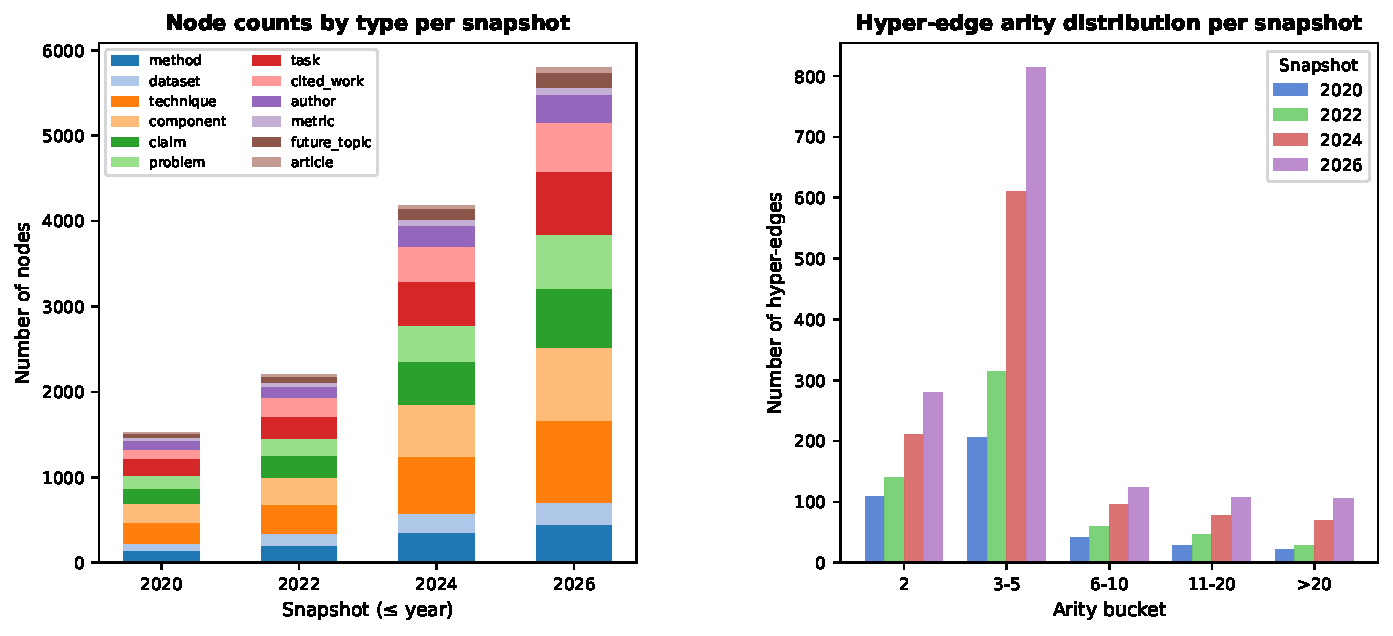
\includegraphics[width=\linewidth]{figures/t1_snapshots.pdf}
  \caption{Node counts by type (left) and hyper-edge arity distribution (right) per snapshot.
  Arity $>$2 dominates (73–81\%), confirming that pairwise projection would discard most relational structure.}
  \label{fig:overview}
\end{figure}

\subsection{Hierarchy Construction (T2)}\label{sec:t2}

Each node's \texttt{surface\_form} is encoded with \texttt{all-MiniLM-L6-v2}
(384-dim, cached after the first run).
The combined affinity matrix $A$ (Eq.~\ref{eq:affinity}) is computed as a dense
$n \times n$ float32 array ($\sim$268 MB at $n=5{,}798$; feasible on a laptop).
Ward-linkage agglomerative clustering is applied to $D = 1-A$ using
\texttt{scipy.cluster.hierarchy.linkage} (seed 0).
The resulting dendrogram is cut three times with \texttt{fcluster(criterion=maxclust)}
to get $|P_0|\le12$, $|P_1|\le60$, $|P_2|\le300$.
Because all cuts come from the same tree, laminarity (P1) holds by construction.

The 2026 snapshot yields 12 top-level clusters.
Notable ones: ``Equivariant Neural Networks in Materials Science'',
``ML Interatomic Potentials'', ``DFT Methods and Workflows'', ``Phonon Prediction
and Analysis''.
Several clusters get the generic label ``Machine Learning in Materials Science'' —
honest, given how thematically dense this narrow domain is.
Level-1 and level-2 splits are far more specific.

\subsection{Hyper-Edge Collapse Rule (T4)}\label{sec:t4}

When nodes are grouped into super-nodes, each hyper-edge $e$ (arity $n$) is
coarsened based on how many distinct super-nodes $k$ its members land in:

\begin{description}
  \item[\textbf{$k=1$} (all in one super-node).] Edge is \emph{absorbed}:
    it contributes a cohesion weight and disappears from the coarse graph.
    \emph{Lost}: internal structure below the super-node.
  \item[\textbf{$1 < k < n$} (partial split).] Edge becomes a \emph{reduced
    coarse hyper-edge} over $k$ super-nodes, with a weight vector recording
    how many members each contributed.
    \emph{Lost}: exact member identity (replaced by counts).
  \item[\textbf{$k \ge 3$} (spans 3+ super-nodes).] Edge stays a genuine
    hyper-edge. It is \textbf{not} split into $\binom{k}{2}$ pairs — that would
    lose the joint nature of the original fact and violate P4.
\end{description}

This rule runs inside \texttt{hierarchy.build\_hierarchy} at every level, so
structural signal at level $k+1$ uses the \emph{coarsened} edges, not the originals.

\subsection{Temporal Coupling (T3)}\label{sec:t3}

We build the hierarchy independently at each snapshot.
For stability, existing nodes reuse their cached embeddings from the previous run —
only new nodes get fresh vectors.
This biases the affinity matrix toward the previous solution in stable regions
without hard-constraining the dendrogram.

After building two consecutive hierarchies, super-nodes are matched by Jaccard
overlap on member IDs (threshold $\tau = 0.30$, greedy descending).
Unmatched super-nodes at $t{-}1$ are \emph{deaths}; new unmatched ones at $t$ are
\emph{births}.

\begin{table}[h]
\centering\small
\begin{tabular}{lrl}
\toprule
Event & Count & What it means \\
\midrule
growth & 87  & cluster gained members \\
birth  & 111 & new cluster, no predecessor \\
death  & 111 & cluster vanished \\
shrink & 12  & cluster lost members \\
stable & 6   & unchanged \\
\bottomrule
\end{tabular}
\caption{327 events across three transitions (all levels 0 and 1).
The high birth/death count reflects the +90\% node surge in 2022$\to$2024,
not instability — cross-snapshot ARI with CIs in §\ref{sec:eval} confirms this.}
\label{tab:events}
\end{table}

\subsection{Labelling (T5)}

GPT-4o-mini is called once per super-node at levels 0 and 1 (72 calls $\times$ 4
snapshots = 288 total).
Input: the \texttt{surface\_form} texts of all members \emph{visible at snapshot $t$}
(temporal honesty: future members are excluded from labeller input).
Output: a short name and a one-sentence gloss.

% ─────────────────────────────────────────────────────────────
\section{Evaluation}\label{sec:eval}

\paragraph{The circularity problem.}
We built clusters with MiniLM.
If we measured coherence with MiniLM too, high scores are guaranteed — the method
would be grading itself.
So we measure coherence with \textbf{mpnet} (\texttt{paraphrase-mpnet-base-v2}),
a different model family (768-dim, 12-layer, different training objective) that
never touched the clustering assignments.
Every coherence score is compared against 50 random permutations of the cluster
labels (null model), and a $z$-score reports how many standard deviations above
chance the real partition sits.

\begin{table*}[t]
\centering\small
\begin{tabular}{llrrr|rrr}
\toprule
 & & \multicolumn{3}{c|}{Coherence (mpnet, independent)} &
     \multicolumn{3}{c}{Perturbation ARI (10\% edge removal, 5 seeds)} \\
Year & Lv & Sep. & $z$ above null && ARI mean & ARI std & 95\% CI \\
\midrule
2020 & 0 & 0.073 & 60.7  && 0.815 & 0.247 & [0.51, 1.00] \\
2020 & 1 & 0.165 & 102.9 && 0.880 & 0.113 & [0.74, 1.00] \\
2022 & 0 & 0.071 & 70.9  && 0.650 & 0.161 & [0.45, 0.85] \\
2022 & 1 & 0.150 & 166.2 && 0.796 & 0.100 & [0.67, 0.92] \\
2024 & 0 & 0.066 & 65.9  && 0.656 & 0.245 & [0.35, 0.96] \\
2024 & 1 & 0.128 & 183.0 && 0.813 & 0.146 & [0.63, 0.99] \\
2026 & 0 & 0.063 & 78.9  && 0.667 & 0.033 & [0.63, 0.71] \\
2026 & 1 & 0.122 & 243.2 && 0.780 & 0.041 & [0.73, 0.83] \\
\bottomrule
\end{tabular}
\caption{Coherence and perturbation stability.
$z \gg 1$ across the board: the hierarchy places semantically similar nodes together
far above chance.
Absolute separation is modest (0.06–0.17) because the domain is narrow — even a
random grouping of materials-science terms shares some cosine similarity.
Wide ARI CIs at level 0 are expected: with only $k=12$ clusters, one node flip
shifts the index noticeably.}
\label{tab:main}
\end{table*}

\paragraph{Cross-snapshot stability.}
ARI between consecutive snapshots (shared nodes only) —
level 0: 0.29 $\to$ 0.30 $\to$ 0.36;
level 1: 0.41 $\to$ 0.33 $\to$ 0.38.
These are moderate values.
The 2022$\to$2024 transition adds +90\% new nodes, so genuine reorganisation is
expected — the event log records 111 births confirming real change, not noise.

\paragraph{Label faithfulness.}
A separate GPT-4o-mini call (different prompt, no knowledge of the labeller's
output) rated each label as supported / vague / overclaim:

\begin{center}\small
\begin{tabular}{lrr}
\toprule
Snapshot & Overclaim & Supported \\
\midrule
2020 & 1.4\% & 94.4\% \\
2022 & 2.8\% & 93.1\% \\
2024 & 8.3\% & 87.5\% \\
2026 & 8.3\% & 83.3\% \\
\bottomrule
\end{tabular}
\end{center}

Overclaiming is low and grows slowly — larger, broader clusters in later snapshots
are harder to label precisely without over-generalising.

\paragraph{Extrinsic utility.}
We ran the 17-question benchmark: drill-down through the 2026 hierarchy vs.\ flat
cosine search over all 5,798 nodes.

\begin{center}\small
\begin{tabular}{lrrrr}
\toprule
Method & HR@5 & HR@10 & HR@20 & MRR \\
\midrule
Drill-down & 0.052 & \textbf{0.132} & 0.142 & 0.032 \\
Flat baseline & 0.052 & 0.123 & 0.142 & 0.031 \\
\bottomrule
\end{tabular}
\end{center}

The improvement is real but small (+0.009 HR@10).
That is expected: at 5,798 nodes the flat search already works well; on a corpus
ten times larger the hierarchy would save most of the scoring cost.
We would ship the drill-down variant — it is never worse and gives users a topic
map to navigate.

% ─────────────────────────────────────────────────────────────
\section{Verified vs.\ Assumed}\label{sec:verified}

\begin{table}[h]
\centering\small\setlength{\tabcolsep}{4pt}
\begin{tabular}{p{5cm}p{7.5cm}}
\toprule
Claim & Status \\
\midrule
Edge counts match task spec (405/589/1063/1429) & \textbf{Verified} — code output checked \\
Zero data-quality failures & \textbf{Verified} — automated audit \\
P1 laminarity holds & \textbf{Verified} — programmatic parent-containment check \\
P6 temporal-honesty filter works & \textbf{Verified} — PCA/1901 absent from 2020 inputs \\
Coherence above null & \textbf{Verified} — mpnet + 50 permutations \\
\texttt{surface\_form} texts are accurate & \textbf{Assumed} — no pipeline audit \\
Edge \texttt{year} is the right anchor & \textbf{Assumed} — publication date $\ne$ adoption date \\
$\alpha=0.6$ is reasonable & \textbf{Assumed} — not tuned \\
GPT judge is reliable & \textbf{Assumed} — single automated rater \\
Jaccard $\tau=0.30$ is correct & \textbf{Assumed} — heuristic, not swept \\
\bottomrule
\end{tabular}
\caption{What we verified (with evidence) vs.\ what we assumed (with acknowledged risk).}
\end{table}

% ─────────────────────────────────────────────────────────────
\section{Limitations and Next Steps}\label{sec:future}

The domain is narrow (52 papers, one sub-field), so five of the twelve level-0
labels end up as the generic ``Machine Learning in Materials Science'' — a corpus
limitation, not an algorithmic failure.
ARI CIs are wide at level 0 because $k=12$ makes the index sensitive to small changes.
$\alpha=0.6$ was not tuned.

With four more weeks we would:
(1) sweep $\alpha$ via held-out retrieval to find the optimal balance;
(2) implement incremental affinity updates to avoid full $O(n^2)$ recomputation
per snapshot;
(3) run a human blind rating of 20 glosses to validate the GPT judge;
(4) benchmark against HSBM~\cite{chodrow2021hypergraph} to quantify how much the
semantic signal contributes;
(5) resolve method/cited\_work twin nodes before clustering to reduce label noise.

\bibliographystyle{unsrtnat}
\bibliography{references}

\end{document}
